% !TEX TS-program = XeLaTeX
% use the following command:
% all document files must be coded in UTF-8
\documentclass[portuguese]{textolivre}
% build HTML with: make4ht -e build.lua -c textolivre.cfg -x -u article "fn-in,svg,pic-align"

\journalname{Texto Livre}
\thevolume{17}
%\thenumber{1} % old template
\theyear{2024}
\receiveddate{\DTMdisplaydate{2023}{8}{31}{-1}} % YYYY MM DD
\accepteddate{\DTMdisplaydate{2023}{11}{26}{-1}}
\publisheddate{\DTMdisplaydate{2023}{12}{20}{-1}}
\corrauthor{Jing Zhang}
\articledoi{10.1590/1983-3652.2024.47754}
%\articleid{NNNN} % if the article ID is not the last 5 numbers of its DOI, provide it using \articleid{} commmand 
% list of available sesscions in the journal: articles, dossier, reports, essays, reviews, interviews, editorial
\articlesessionname{dossier}
\runningauthor{Zhang e You}
%\editorname{Leonardo Araújo} % old template
\sectioneditorname{Daniervelin Pereira}
\layouteditorname{Leonado Araújo}

\title{Corpus de aprendizes de português da Universidade de Macau e ensino de português L2}
\othertitle{University of Macau Portuguese learner corpus and teaching of Portuguese L2}
% if there is a third language title, add here:
%\othertitle{Artikelvorlage zur Einreichung beim Texto Livre Journal}

\author[1]{Jing Zhang~\orcid{0000-0003-4801-6354}\thanks{Email: \href{mailto:jingz@um.edu.mo}{jingz@um.edu.mo}}}
\author[1]{Mu You~\orcid{0000-0001-5029-3903}\thanks{Email: \href{mailto:youmuafonso@gmail.com}{youmuafonso@gmail.com}}}
\affil[1]{Universidade de Macau, Faculdade de Letras, Departamento de Português, Macau, China.}

\addbibresource{article.bib}
% use biber instead of bibtex
% $ biber article

% used to create dummy text for the template file
\definecolor{dark-gray}{gray}{0.35} % color used to display dummy texts
\usepackage{lipsum}
\SetLipsumParListSurrounders{\colorlet{oldcolor}{.}\color{dark-gray}}{\color{oldcolor}}

%cites: multiple citation
%\usepackage{cite}
%\makeatletter
%\newcommand{\citecomment}[2][]{\citen{#2}#1\citevar}
%\newcommand{\citeone}[1]{\citecomment{#1}}
%\newcommand{\citetwo}[2][]{\citecomment[,~#1]{#2}}
%\newcommand{\citevar}{\@ifnextchar\bgroup{;~\citeone}{\@ifnextchar[{;~\citetwo}{]}}}
%\newcommand{\citefirst}{\@ifnextchar\bgroup{\citeone}{\@ifnextchar[{\citetwo}{]}}}
%\newcommand{\cites}{[\citefirst}
%\makeatother

%table footnote
%\usepackage{tablefootnote}
% used here only to provide the XeLaTeX and BibTeX logos
\usepackage{hologo}

% if you use multirows in a table, include the multirow package
\usepackage{multirow}

% provides sidewaysfigure environment
\usepackage{rotating}

% CUSTOM EPIGRAPH - BEGIN 
%%% https://tex.stackexchange.com/questions/193178/specific-epigraph-style
\usepackage{epigraph}
\renewcommand\textflush{flushright}
\makeatletter
\newlength\epitextskip
\pretocmd{\@epitext}{\em}{}{}
\apptocmd{\@epitext}{\em}{}{}
\patchcmd{\epigraph}{\@epitext{#1}\\}{\@epitext{#1}\\[\epitextskip]}{}{}
\makeatother
\setlength\epigraphrule{0pt}
\setlength\epitextskip{0.5ex}
\setlength\epigraphwidth{.7\textwidth}
% CUSTOM EPIGRAPH - END

% LANGUAGE - BEGIN
% ARABIC
% for languages that use special fonts, you must provide the typeface that will be used
% \setotherlanguage{arabic}
% \newfontfamily\arabicfont[Script=Arabic]{Amiri}
% \newfontfamily\arabicfontsf[Script=Arabic]{Amiri}
% \newfontfamily\arabicfonttt[Script=Arabic]{Amiri}
%
% in the article, to add arabic text use: \textlang{arabic}{ ... }
%
% RUSSIAN
% for russian text we also need to define fonts with support for Cyrillic script
% \usepackage{fontspec}
% \setotherlanguage{russian}
% \newfontfamily\cyrillicfont{Times New Roman}
% \newfontfamily\cyrillicfontsf{Times New Roman}[Script=Cyrillic]
% \newfontfamily\cyrillicfonttt{Times New Roman}[Script=Cyrillic]
%
% in the text use \begin{russian} ... \end{russian}
% LANGUAGE - END

% EMOJIS - BEGIN
% to use emoticons in your manuscript
% https://stackoverflow.com/questions/190145/how-to-insert-emoticons-in-latex/57076064
% using font Symbola, which has full support
% the font may be downloaded at:
% https://dn-works.com/ufas/
% add to preamble:
% \newfontfamily\Symbola{Symbola}
% in the text use:
% {\Symbola }
% EMOJIS - END

% LABEL REFERENCE TO DESCRIPTIVE LIST - BEGIN
% reference itens in a descriptive list using their labels instead of numbers
% insert the code below in the preambule:
%\makeatletter
%\let\orgdescriptionlabel\descriptionlabel
%\renewcommand*{\descriptionlabel}[1]{%
%  \let\orglabel\label
%  \let\label\@gobble
%  \phantomsection
%  \edef\@currentlabel{#1\unskip}%
%  \let\label\orglabel
%  \orgdescriptionlabel{#1}%
%}
%\makeatother
%
% in your document, use as illustraded here:
%\begin{description}
%  \item[first\label{itm1}] this is only an example;
%  % ...  add more items
%\end{description}
% LABEL REFERENCE TO DESCRIPTIVE LIST - END


% add line numbers for submission
%\usepackage{lineno}
%\linenumbers

\begin{document}
\maketitle

\begin{polyabstract}
\begin{abstract}
O presente artigo apresenta um \textit{corpus} de aprendizes chineses de português L2 com a anotação de \textit{PoS} e lema, destacando-se sua potencialidade de análise quantitativa e qualitativa na identificação de padrões linguísticos dos aprendizes, contribuindo, dessa forma, para o ensino de português L2. Este \textit{corpus} (Corpus de Aprendizes de Português da Universidade de Macau), denominado UMPLC, contém, no total, 933 composições produzidas por 122 estudantes de português da Universidade de Macau durante três anos de estudo consecutivos. A anotação de \textit{PoS} e lema realizou-se através do Stanza, anotador automático desenvolvido por \textcite{qi2020stanza}. A fim de garantir a consistência de anotação, o resultado foi revisado manualmente. Nesta pesquisa, as informações de \textit{PoS} e lema permitem-nos investigar quantitativa e qualitativamente diversos fenômenos existentes no \textit{corpus} relativos ao aspeto lexical e à mudança diacrônica desse aspeto. Dois estudos foram realizados com base em uma abordagem contrastiva, comparando-se o português dos aprendizes do \textit{corpus} com o português nativo. Foram descobertas características de não-natividade linguística desses aprendizes, o que permitirá que os professores de português L2 se concentrem nas áreas em que é necessário um trabalho corretivo. 

\keywords{\textit{Corpus} de aprendizes \sep Aprendizes chineses de português L2 \sep Análises quantitativas e qualitativas\sep Aplicações pedagógicas}
\end{abstract}

\begin{english}
\begin{abstract}
This article presents a corpus of Chinese learners of Portuguese L2 with \textit{PoS} and lemma annotations, highlighting its potential for quantitative and qualitative analysis in identifying linguistic patterns among learners, thus contributing to the teaching of Portuguese L2. This corpus (University of Macau Portuguese Learners Corpus), named UMPLC, contains a total of 933 compositions produced by 122 Portuguese students from University of Macau over three consecutive years of study. PoS and lemma annotation was performed using Stanza, an automatic annotator developed by \textcite{qi2020stanza}. To ensure annotation consistency, the results were manually reviewed. In this research, the PoS and lemma information enables us to quantitatively and qualitatively investigate various phenomena in the corpus relating to lexical aspects and diachronic changes in this regard. Two studies were conducted based on a contrastive approach, comparing the Portuguese of learners in the corpus with native Portuguese. Non-native linguistic characteristics were discovered, allowing Portuguese L2 teachers to focus on areas requiring corrective work.

\keywords{Learner corpus \sep Chinese learners of Portuguese L2\sep Quantitative and qualitative analysis \sep Pedagogical applications}
\end{abstract}
\end{english}
% if there is another abstract, insert it here using the same scheme
\end{polyabstract}

\section{Introdução}\label{sec-intro}
A ideia de coletar produções linguísticas de aprendizes não é nova, mas a compilação de \textit{corpora} de aprendizes (CA) eletrônicos é um fenômeno relativamente recente, que teve início no final dos anos 1980 e início dos anos 1990 \cite[p. 128]{nesselhauf2004learner}[p. 5]{Granger2002bird}. Com o auxílio de computadores, esse tipo de \textit{corpus} apresenta duas vantagens significativas \parencite{granger_gilquin_meunier_2015}. Primeiramente, devido à sua grande escala, os dados são mais representativos do que aqueles que envolvem apenas um número limitado de aprendizes. Em segundo lugar, por estarem em formato eletrônico, os dados podem ser analisados com ferramentas de pesquisa que aceleram a observação e permitem um amplo escopo de estudos que não podem ser realizados manualmente ou apenas com um custo considerável em termos de recursos humanos. Essa natureza eletrônica dos CA permite que os resultados de pesquisa sejam compartilhados e verificados de forma eficiente e confiável \parencite[p. 130]{nesselhauf2004learner}. Além disso, os dados anotados facilitam consideravelmente as análises linguísticas.

Os CA são frequentemente associados à análise da interlíngua dos aprendizes, servindo como base para descobrir padrões gerais da interlíngua \cite{cobb2013,nesselhauf2004learner,santos2016corpus} e revelando as fases do desenvolvimento linguístico e competência transitória \parencite{selinker1992rediscovering}, o que pode facilitar a adaptação do ensino de línguas não maternas. \textcite{rundell1996corpus} enfatiza esse significado óbvio dos CA, considerando que esses \textit{corpora} fornecem informações confiáveis sobre o uso da língua pelos aprendizes, indicando suas dificuldades típicas. Os CA, para \textcite{granger1998}, desempenham um papel vital no \textit{design} de ferramentas de ensino de inglês, que podem ser aprimoradas com dados de falantes nativos. Esses dados fornecem informações sobre o que é típico em inglês, enquanto os dados dos não-falantes nativos destacam o que é desafiador para os aprendizes em geral e para grupos específicos de aprendizes.

Um \textit{corpus} de aprendizes pode contribuir de diversas maneiras para os objetivos acadêmicos e pedagógicos. Aqui, destacam-se as aplicações dos CA para diversos fins pedagógicos: i) elaboração, com base em CA, de dicionários\footnote{Há vários dicionários baseado em CA dedicados à língua inglesa \cite[p. 136]{granger2004computer}[p. 137]{nesselhauf2004learner}, tais como o \textit{Longman Essential Activator}, o \textit{Longman Dictionary of Contemporary English}, o \textit{Cambridge International Dictionary of English}, o \textit{Cambridge Advanced Learner’s Dictionary}, entre outros. No que diz respeito à língua portuguesa, destaca-se o \textit{A frequency dictionary of Portuguese} \cite{Dic2008}, que é baseado em um \textit{corpus} de falantes nativos.}, gramáticas\footnote{\href{http://www.telenex.hku.hk/telec/pmain/opening.htm}{TeleNex} e o \textit{Longman dictionary of common errors} \cite{turton1996longman} são dois exemplos.} e outros materiais didáticos adequados a diferentes perfis de aprendizes \cite{granger2004computer,nesselhauf2004learner,santos2016corpus}; 
ii) \textit{design} de programas de ensino que considerem tanto as informações de frequência lexical quanto as dificuldades identificadas por meio da análise de corpora de aprendentes e de falantes nativos \cite[p. 22-23]{Granger2002bird}; iii) implementação de metodologias de ensino, incluindo a aprendizagem orientada por dados (\textit{data-driven learning}). \textcite{Grangertribble1998} argumentam que os CA e corpora de falantes nativos proporcionam aos aprendizes oportunidades para explorar diretamente os fatos linguísticos, estimulando seu aprendizado. Ademais, as descobertas da pesquisa com CA podem ser incorporadas às atividades pedagógicas, oferecendo informações cruciais sobre o que deve ser ensinado e como ensinar \cite[p. 139]{nesselhauf2004learner}.

O campo de pesquisa dos CA tem experimentado um notável desenvolvimento. O \href{https://uclouvain.be/en/research-institutes/ilc/cecl/learner-corpora-around-the-world.html}{\textit{Learner Corpora Around the World}},  organizado pela Universidade Católica de Lovaina, contém 200 CA, dos quais 176 (88\%) são \textit{corpora} monolíngues (102 em inglês e 74 em outras línguas), e 23 (11,4\%) são bilíngues ou multilíngues. Entre os CA publicados, destacam-se cinco relacionados ao português, sendo dois monolíngues (o \textit{Learner Corpus of Portuguese L2} (COPLE2), da Universidade de Lisboa; o Corpus Oral de Português como Língua Adicional-Brasil, da Universidade de Limerick, em desenvolvimento) e três bilíngues/multilíngues (o \textit{Multlingual Academic Corpus of Assignments} - \textit{Writing and Speech} (MACAWS) – Português/Russo, da Universidade de Arizona; o \textit{Multilingual Corpus of Second Language Speech} (MuSSeL) – Chinês Mandarim, Francês, Português e Espanhol, da Universidade de Utah; o \textit{Leiden Learner Corpus} – Holandês, Francês, Italiano, Português e Espanhol, da Universidade de Leiden.  Além do primeiro \textit{corpus} monolíngue em português anteriormente mencionado, salienta-se ainda \href{https://teitok2.iltec.pt/peapl2/#http://teitok.iltec.pt/peapl2/}{o Corpus de Produções Escritas de Aprendentes de PL2} (PEAPL2) da Universidade de Coimbra. Ambos compartilham características comuns, consistindo em dados sincrônicos produzidos por falantes de diferentes línguas maternas, incluindo o chinês. 

Na China, o primeiro \textit{corpus} de aprendizes chineses, conhecido como o Corpus de Aprendizes Chineses de Inglês (CLEC), foi criado em 1999 pelas Universidades de Estudos Estrangeiros de Guangdong e de Jiaotong de Xangai \cite[62]{yang2001}. Esse \textit{corpus} é composto por materiais escritos por estudantes de Inglês Profissional, Inglês Universitário e Inglês do Ensino Secundário. Desde então, surgiram outros CA, que predominantemente representam produções em inglês. Simultaneamente, a abordagem metodológica baseada em CA também tem se desenvolvido.

No que diz respeito à língua portuguesa, não há registros de existência de um \textit{corpus} de aprendizes chineses na China. Nossa pesquisa busca preencher essa lacuna por meio da construção de um \textit{corpus} de produções escritas em português L2. Nas seções seguintes, descreveremos esse \textit{corpus} e suas características quantitativas, bem como suas aplicações pedagógicas.

\section{Construção de um \textit{corpus} de aprendizes chineses de português L2}\label{sec aprensetação}

Nesta seção, abordamos a contextualização da pesquisa, o \textit{design} do \textit{corpus}, a coleta e documentação de dados, assim como sua estruturação e a anotação. 

\subsection{Contextualização da pesquisa}
Devido ao fortalecimento das relações entre a China e os países de língua portuguesa, estamos testemunhando um crescimento significativo na demanda por profissionais que dominam bem a língua portuguesa. \textcite{Grosso2021}, no Referencial para o Ensino de Português Língua Estrangeira na China, destacam que o português é considerado uma das línguas não comuns\footnote{Conforme mencionado por \textcite{Yan2019}, o termo 'línguas não comuns' refere-se às línguas estrangeiras excluindo o inglês, russo, japonês, francês, alemão, espanhol e árabe. Esse conceito foi criado para simplificar a organização e a administração do ensino de idiomas.} mais procuradas na China Interior. 

Em Macau, o português, cujo estatuto oficial é garantido pela \href{https://bo.io.gov.mo/bo/i/1999/leibasica/index.a}{Lei Básica da Região Administrativa Especial de Macau}, continua sendo principalmente utilizado na administração pública e no sistema judicial. No entanto, não é frequentemente utilizado na vida cotidiana dos residentes de Macau. De acordo com dados estatísticos fornecidos pela Direção dos Serviços de Estatística e Censos de Macau\footnote{Disponível em \href{https://www.dsec.gov.mo/getAttachment/fda23546-c321-47ae-a5b3-b4a5071cf732/P_CEN_PUB_2021_Y.aspx}{Resultados Globais dos Censos 2021.}}, em termos de domínio geral de línguas, 86,2\% da população fala fluentemente cantonês como meio de comunicação, 45,0\% fala mandarim, 22,7\% fala inglês e 2,3\% fala português. 


Para os jovens de Macau, o ensino universitário representa uma das principais oportunidades para aprenderem português. Atualmente, há uma justificativa clara para o aumento de cursos de língua portuguesa, bem como o crescimento do número de estudantes chineses de português, tanto na China Interior quanto em Macau. O referencial mencionado anteriormente lista 52 instituições de ensino superior que oferecem cursos de português na China Interior e seis em Macau.

Com o maior departamento de ensino de português na Ásia e excelentes condições acadêmicas, a Universidade de Macau atrai jovens chineses de Macau e da China Interior para aprenderem português. Isso a coloca em uma posição ideal para desenvolver um projeto de pesquisa sobre a construção e aplicação do \textit{corpus} de aprendizes de português L2. Um dos fatores a serem considerados é a regularidade do aprendizado de estudantes universitários que produzem materiais linguísticos de forma sistemática, o que pode tornar a pesquisa em questão mais produtiva.

Neste contexto, o Departamento de Português e o Laboratório de Processamento de Linguagem Natural e Tradução Automática Português-Chinês da Universidade de Macau iniciaram conjuntamente o projeto Corpus de Aprendizes Chineses de Português L2 (UMPLC) no primeiro semestre do ano letivo 2018/2019, e sua conclusão está prevista para o segundo semestre do ano letivo 2023/2024. 


\subsection{\textit{Design} do UMPLC}
O UMPLC, composto por produções escritas de aprendizes adultos chineses de português L2 matriculados no ensino superior, tem como objetivo criar uma plataforma que ofereça ferramentas de pesquisa sobre o processo e os resultados do ensino e da aquisição de L2. Atualmente, encontra-se na fase final de desenvolvimento.

O projeto envolve 122 alunos matriculados no Curso de Licenciatura ou no Curso de Minor em Estudos Portugueses da Universidade de Macau, os quais são provenientes de Macau e da China Interior e têm o chinês como língua materna. Dentre esses alunos, 47 participaram de todas as onze etapas diferentes de coleta de dados ao longo dos seus primeiros três anos de estudo, nos quais frequentaram disciplinas de compreensão e produção escrita em português L2. Devido à existência de um nível de proficiência linguística estabelecido de acordo com a organização curricular dos cursos, que os alunos devem alcançar no final de cada ano de estudo, é possível avaliar as competências linguísticas dos informantes em cada fase da coleta de dados. Assim, trata-se de dados diacrônicos, que podem fornecer evidências das diferentes etapas na evolução da língua \cite{kubler2015corpus}.

Cada participante é solicitado a preencher um formulário de informações pessoais. Os dados coletados, apresentados na Tabela \ref{Tab 1}, são posteriormente integrados aos metadados do corpus.
\begin{table}[htbp]
\centering
\begin{threeparttable}
\caption{Perfis dos participantes.}
\label{Tab 1}
\begin{tabular}{ll}
\toprule
Número total de participantes  & 122                                                                                                                          \\ 
Instituição de ensino superior & Universidade de Macau                                                                                                        \\ 
Curso que frequentam           & \begin{tabular}[c]{@{}l@{}}Curso de Licenciatura em Estudos Portugueses\\ Curso de \textit{Minor} em Estudos Portugueses\end{tabular} \\
Contexto de aprendizado        & Português   L2                                                                                                               \\ 
Idade                          & 18 a 22 anos                                                                                                                 \\ 
Língua materna                 & Chinês                                                                                                                       \\ 
Origem                         & Macau e China Interior                                                                                                       \\ 
\bottomrule
\end{tabular}
\source{Autoria própria.}
\end{threeparttable}
\end{table}

\subsection{Coleta e documentação de dados}
Os dados consistem em avaliações textuais (realizadas em testes, exames semestrais e finais) produzidas pelos estudantes dentro da sala de aula, sem acesso a dicionários ou livros de referência e dentro de um limite de tempo. Esses dados se apresentam em duas formas: a maioria são textos manuscritos, enquanto uma pequena parte são textos eletrônicos\footnote{O 8º momento da coleta de dados coincidiu com o período da pandemia da Covid-19, o que levou os estudantes da Universidade de Macau a realizar as avaliações de forma \textit{online}.}. Os manuscritos foram inicialmente digitalizados e armazenados em formato PDF e, posteriormente, transcritos manualmente. A tentativa de obtenção automática de arquivos digitais através de OCR não foi bem-sucedida devido à natureza manuscrita dos textos.

A etapa mais demorada do processo é a coleta de textos, que ocorreu ao longo de três anos letivos e seis semestres, de 2018 a 2021. Todos os dados foram digitados manualmente e passaram por uma verificação ortográfica realizada por um grupo de assistentes, composto por mestrandos e doutorandos dos cursos de Linguística Aplicada (Português) e Tradução Português-Chinês. Posteriormente, esses dados foram anotados com informações linguísticas, divididas em duas estruturas: \textit{PoS} (\textit{Part of Speech}) e lema (a forma canônica da palavra). Além disso, os dados originais passaram por correções linguísticas providenciadas por professores de Português, que são falantes nativos da língua.

Dessa forma, este conjunto de dados disponibiliza cinco tipos distintos de informações: dados originais gravados em PDF, dados transcritos digitalmente, que permanecem idênticos aos originais, dados com correções ortográficas, dados anotados linguisticamente e dados com correções linguísticas.

\subsection{Estruturação do UMPLC}
Os metadados dividem-se em duas partes distintas. A primeira parte está relacionada aos dados pessoais dos participantes, conforme apresentado na Tabela 1. A segunda parte abrange informações sobre os textos. A Tabela 2 revela que o \textit{corpus} abrange um total de 933 textos, contendo 171914
 palavras. Esses textos foram coletados em onze momentos diferentes, abrangendo um período de três anos e seis semestres. No primeiro ano, foram registrados cinco momentos, enquanto no segundo e terceiro ano, foram registrados três momentos em cada. Nos dois últimos momentos, foram abordados dois temas distintos em cada ocasião, e o tempo de avaliação dobrou em relação aos períodos anteriores. Diante dessa configuração, os textos com temas diferentes foram agrupados em subconjuntos separados, resultando, assim, em quatro subcorpora: CA10A, CA10B, CA11A e CA11B. Com base nas metas estabelecidas para cada ano de estudo, os estudantes que completarem o segundo ano alcançarão o nível Intermediário no sistema Celpe-Bras. Já os que concluírem o terceiro ano atingirão o nível Intermediário Superior.

Os textos coletados são narrativos, argumentativos e descritivos, abordando uma variedade de tópicos definidos pelos professores que ministram as disciplinas de Compreensão e Produção Escrita em Língua Portuguesa. Esses textos refletem, assim, o aprendizado dos alunos na sala de aula. As informações sobre os textos que compõem o \textit{corpus} são apresentadas na Tabela \ref{Tab2}.

\begin{table}[h]
\footnotesize
\begin{threeparttable}
\caption{Informações básicas do UMPLC.}
\label{Tab2}
\begin{tabular}{cccccccc}
\toprule
Momento             & 
\multicolumn{1}{p{1.4cm}}{Título de subcorpus} & 
\multicolumn{1}{p{1.4cm}}{Tipo de texto} & 
\multicolumn{1}{p{1.4cm}}{Número de texto} & 
\multicolumn{1}{p{1.4cm}}{Número de palavra} & 
\multicolumn{1}{p{1.4cm}}{Data de coleta} & 
\multicolumn{1}{p{1.4cm}}{Ano\_Se\-mes\-tre em que estão os participantes} & 
\multicolumn{1}{p{1.4cm}}{Nível de proficiência - Celpe-Bras} \\ 
\midrule
1                   & CA1                                                               & Descritivo                                                  & 82                                                            & 12245                                                           & 06/11/2018                                                   & 1\_1                                                                                      & ---                                                                           \\
2                   & CA2                                                               & Narrativo                                                   & 82                                                            & 15474                                                           & 12/12/2018                                                   & 1\_1                                                                                      & ---                                                                           \\
3                   & CA3                                                               & Narrativo                                                   & 67                                                            & 9922                                                            & 27/02/2019                                                   & 1\_2                                                                                      & ---                                                                           \\
4                   & CA4                                                               & Narrativo                                                   & 70                                                            & 10014                                                           & 14/03/2019                                                   & 1\_2                                                                                      & ---                                                                           \\
5                   & CA5                                                               & Narrativo                                                   & 70                                                            & 10322                                                           & 09/05/2019                                                   & 1\_2                                                                                      & ---                                                                           \\
6                   & CA6                                                               & Narrativo                                                   & 65                                                            & 11610                                                           & 10/10/2019                                                   & 2\_1                                                                                      & ---                                                                           \\
7                   & CA7                                                               & Argumentativo                                               & 65                                                            & 11869                                                           & 14/12/2019                                                   & 2\_1                                                                                      & ---                                                                           \\
8                   & CA8                                                               & Argumentativo                                               & 61                                                            & 10821                                                           & 30/05/2020                                                   & 2\_2                                                                                      & \parbox[t]{1.4cm}{Intermediário}                                                                 \\
9                   & CA9                                                               & Argumentativo                                               & 67                                                            & 13341                                                           & 19/11/2020                                                   & 3\_1                                                                                      & ---                                                                           \\ 
\multirow{2}{*}{10} & CA10A                                                             & Argumentativo                                               & 68                                                            & 18135                                                           & \multirow{2}{*}{06/12/2020}                                  & \multirow{2}{*}{3\_1}                                                                     & \multirow{2}{*}{---}                                                          \\
                    & CA10B                                                             & Argumentativo                                               & 68                                                            & 12079                                                           &                                                              &                                                                                           &                                                                               \\ 
\multirow{2}{*}{11} & CA11A                                                             & Argumentativo                                               & 84                                                            & 24776                                                           & \multirow{2}{*}{25/05/2021}                                  & \multirow{2}{*}{3\_2}                                                                     & \multirow{2}{*}{\parbox[t]{1.4cm}{Intermediário Superior}}                                       \\
                    & CA11B                                                             & Narrativo                                                   & 84                                                            & 11306                                                           &                                                              &                                                                                           &                                                                               \\ 
Total               & ---                                                               & ---                                                         & 933                                                           & 171914                                                          & ---                                                          & ---                                                                                       & ---                                                                           \\ 
\bottomrule
\end{tabular}
\source{Autoria própria.}
\end{threeparttable}
\end{table}

\subsection{Anotação do UMPLC}

A anotação é um processo interpretativo que adiciona informações linguísticas, como morfológicas, semânticas, sintáticas, discursivas, etc., a textos \cite[2]{garside1997corpus}. Independentemente de ser realizada de forma automática ou não, a anotação fornece o mesmo tipo de informações que as análises linguísticas tradicionais ofereceriam. Em outras palavras, trata-se de uma prática que analisa os textos e fornece os resultados de forma sistemática e acessível \cite[13]{mcenery2011corpus}. Isso significa que um \textit{corpus} anotado possui pelo menos duas vantagens: as informações nele armazenadas não apenas facilitam substancialmente investigações linguísticas, evitando a necessidade de repetir o trabalho árduo de examinar os textos palavra por palavra, mas também estabelecem uma base comum a partir da qual diferentes pesquisas podem ser conduzidas com maior consistência.

O nosso \textit{corpus} atual conta com dois tipos de anotação, \textit{PoS} e lema, que foram realizados seguindo o esquema \href{https://universaldependencies.org}{\textit{Universal Dependencies}} (UD) \cite{de-marneffe-etal-2021-universal}. A escolha do UD foi motivada por duas razões principais. Primeiramente, esse esquema é caracterizado por um conjunto de etiquetas e diretrizes que possibilitam uma anotação consistente entre diferentes idiomas, e até mesmo em todos eles, e permite extensões para línguas específicas\footnote{Para obter informações adicionais, visite o site oficial da UD.}. O UD já foi adotado por 183 \textit{treebanks} em 104 línguas \cite[256]{de-marneffe-etal-2021-universal}, e tanto os \textit{treebanks} quanto os documentos de anotação acumulados durante a sua compilação representam um recurso valioso. Em segundo lugar, o \textit{tagset} do UD é relativamente simples, o que contribui para a qualidade e a rapidez da anotação manual.

A anotação é realizada em duas etapas. A primeira é feita automaticamente com o uso do \href{https://stanfordnlp.github.io/stanza}{Stanza} \cite{qi2020stanza}, uma ferramenta que pode processar textos em 70 idiomas, seguindo o esquema de UD. No entanto, em vez da versão original, optou-se por anotar a versão revisada ortograficamente, uma vez que erros ortográficos geralmente não são relevantes e podem afetar a anotação, resultando em etiquetas incorretas e difíceis de corrigir. Como o Stanza é treinado com dados de falantes nativos, qualquer desvio encontrado nos textos dos aprendizes poderia diminuir a precisão da anotação. Por esse motivo, na segunda etapa, foi realizada uma revisão manual conduzida pelo mesmo grupo de assistentes estudantes mencionado anteriormente. A revisão humana reduziu significativamente os erros de anotação, embora seja inevitável a ocorrência de alguns erros isolados.

Apesar das várias diretrizes relacionadas às possíveis questões linguísticas na anotação de \textit{corpus} em português \cite{de2016universal,rademaker2017universal}, durante a fase de revisão, foi identificado um grande número de problemas não abordados anteriormente. O presente artigo não aborda esses detalhes específicos, no entanto, enfatiza uma modificação significativa no \textit{tagset} do UD. Devido à presença de palavras não convencionais no UMPLC, criadas pelos estudantes ou ilegíveis, foi necessário adicionar uma etiqueta ("UNKNOWN") para marcá-las. No total, foram utilizadas 17 etiquetas para a anotação de \textit{PoS} (ver Tabela \ref{Tab3}). 

\begin{table}[h]
\centering
\begin{threeparttable}
\caption{\textit{Tagset} do UMPLC.}
\label{Tab3}
\begin{tabular}{ll}
\toprule
Etiqueta                        & Exemplos           \\ 
AUX (verbo auxiliar)            & ser, estar         \\ 
ADJ (adjetivo)                  & alto, comprido     \\ 
ADP (preposição)                & de, em             \\ 
ADV (advérbio)                  & não, já            \\ 
CCONJ (conjunção coordenativa)  & e, mas             \\ 
DET (determinante)              & o, um              \\ 
INTJ (interjeição)              & obrigado, olá      \\ 
NOUN (substantivo)              & país, dia          \\ 
NUM (número)                    & 3, 66              \\ 
PRON (pronome)                  & eu, que            \\ 
PROPN (substantivo próprio)     & Sofia, Ronaldo     \\ 
PUNCT (pontuação)               & “, ?               \\ 
SCONJ (conjunção subordinativa) & porque, quando     \\ 
SYM (símbolo)                   & \$, ℃              \\ 
UNKNOWN (palavra inexistente)   & aúnueu, attche     \\ 
VERB (verbo pleno)              & querer, fazer      \\ 
X (palavra estrangeira)         & part-time, cosplay \\ 
\bottomrule
\end{tabular}
\source{Autoria própria.}
\end{threeparttable}
\end{table}

Um \textit{corpus} de aprendizes, especialmente aqueles com anotações, representa um recurso valioso para pesquisas relacionadas ao ensino e aquisição do português L2. Com base no UMPLC e em \textit{corpora} de referência, que incluem o \href{https://www.sketchengine.eu/pttenten-portuguese-corpus/}{ptTenTen20} (\textit{corpus} de português L1 com \textit{c.} 12,5 bilhões de palavras) e o \href{https://www.sketchengine.eu/zhtenten-chinese-corpus/}{zhTenTen17} (\textit{corpus} de chinês L1 com \textit{c.} 13,5 bilhões de palavras), além de três pequenos \textit{corpora} de português L1 desenvolvidos pelos próprios autores, conduziram-se dois estudos. O primeiro concentra-se na análise da variação lexical entre os textos produzidos por falantes nativos e não nativos, enquanto o segundo explora o uso de advérbios, com exemplos de dois deles: "especialmente" e "nomeadamente".

\section{Estudo I: variação lexical }
Para avaliar o vocabulário utilizado pelos aprendizes no UMPLC, empregamos o índice \textit{Type/Token Ratio} (TTR), que mede a variação lexical \cite{wolfe1998}. O TTR é calculado como a relação entre o número de palavras diferentes e o número total de palavras em um texto\footnote{É de notar que a definição de "palavra" não abrange as pontuações neste artigo.}.  Quanto mais elevado o valor, maior a diversidade lexical presente em um determinado texto. 

Para evidenciar eventuais disparidades entre os textos produzidos por falantes nativos e não nativos, além do UMPLC, foram introduzidos cinco subcorpora selecionados aleatoriamente do ptTenTen20, denominados "SUB1", "SUB2", "SUB3", "SUB4" e "SUB5". Além disso, foram utilizados três \textit{corpora} especialmente compilados pelos próprios autores, denominados "CPCOVID", "CPMESSI" e "CPMPOX", para servirem como subcorpora de referência.

O UMPLC está subdividido em 13 subcorpora, designados como "CA1", "CA2", "CA3", "CA4", "CA5", "CA6", "CA7", "CA8", "CA9", "CA10A", "CA10B", "CA11A" e "CA11B", que registram o desempenho dos aprendizes em cada momento de coleta. É importante notar que o valor do TTR é influenciado pela extensão do texto, geralmente diminuindo à medida que os textos se tornam mais longos. Portanto, a escala dos subcorpora de referência foi ajustada para garantir uma comparação justa com os subcorpora do UMPLC.
Os corpora CPCOVID, CPMESSI e CPMPOX consistem em notícias recentes coletadas através do \textit{Google News}, com base nas palavras-chave: "surto de COVID", "Messi campeão" e "surto de Mpox em Portugal". Essa seleção foi feita de modo a cada \textit{corpus} ter um tema específico, permitindo uma comparação significativa entre eles e os subcorpora do UMPLC. No total, foram utilizados 21 subcorpora, dos quais oito são (sub)corpora de referência.
Os dados pertinentes estão resumidos na Tabela \ref{tab4} e ilustrados na Figura \ref{fig 1}.


\begin{table}[h]
\centering
\small
\begin{threeparttable}
\caption{TTRs e dados relevantes dos 21 (sub)corpora.}
\label{tab4}
\begin{tabular}{lllll}
\toprule
(Sub)corpus & Ano\_Semestre & Número de Tipo & Número de Palavra & TTR(\%) \\
\midrule
CA1         & 1\_1          & 416            & 12245             & 3,4     \\ 
CA2         & 1\_1          & 665            & 15474             & 4,3     \\ 
CA3         & 1\_2          & 1403           & 9922              & 14,14   \\ 
CA4         & 1\_2          & 1064           & 10014             & 10,63   \\ 
CA5         & 1\_2          & 1282           & 10322             & 12,42   \\ 
CA6         & 2\_1          & 1929           & 11610             & 16,61   \\ 
CA7         & 2\_1          & 1530           & 11869             & 12,89   \\ 
CA8         & 2\_2          & 1824           & 10821             & 16,86   \\ 
CA9         & 3\_1          & 2114           & 13341             & 15,85   \\ 
CA10A       & 3\_1          & 2370           & 18135             & 13,07   \\ 
CA10B       & 3\_1          & 1539           & 12079             & 12,74   \\ 
CA11A       & 3\_2          & 2804           & 24776             & 11,32   \\ 
CA11B       & 3\_2          & 1199           & 11306             & 10,6    \\ 
SUB1        & —             & 2024           & 7593              & 26,66   \\ 
SUB2        & —             & 2570           & 11347             & 22,65   \\ 
SUB3        & —             & 3605           & 15647             & 23,04   \\ 
SUB4        & —             & 4856           & 22168             & 21,91   \\ 
SUB5        & —             & 5343           & 25628             & 20,85   \\ 
CPCOVID     & —             & 2328           & 9434              & 24,68   \\ 
CPMESSI     & —             & 1687           & 8220              & 20,52   \\ 
CPMPOX      & —             & 1587           & 10329             & 15,36   \\   
\bottomrule
\end{tabular}%
\source{Autoria própria.}
\end{threeparttable}
\end{table}

\begin{figure}
    \centering
    \label{Fig 1}
    \begin{minipage}{1\textwidth} 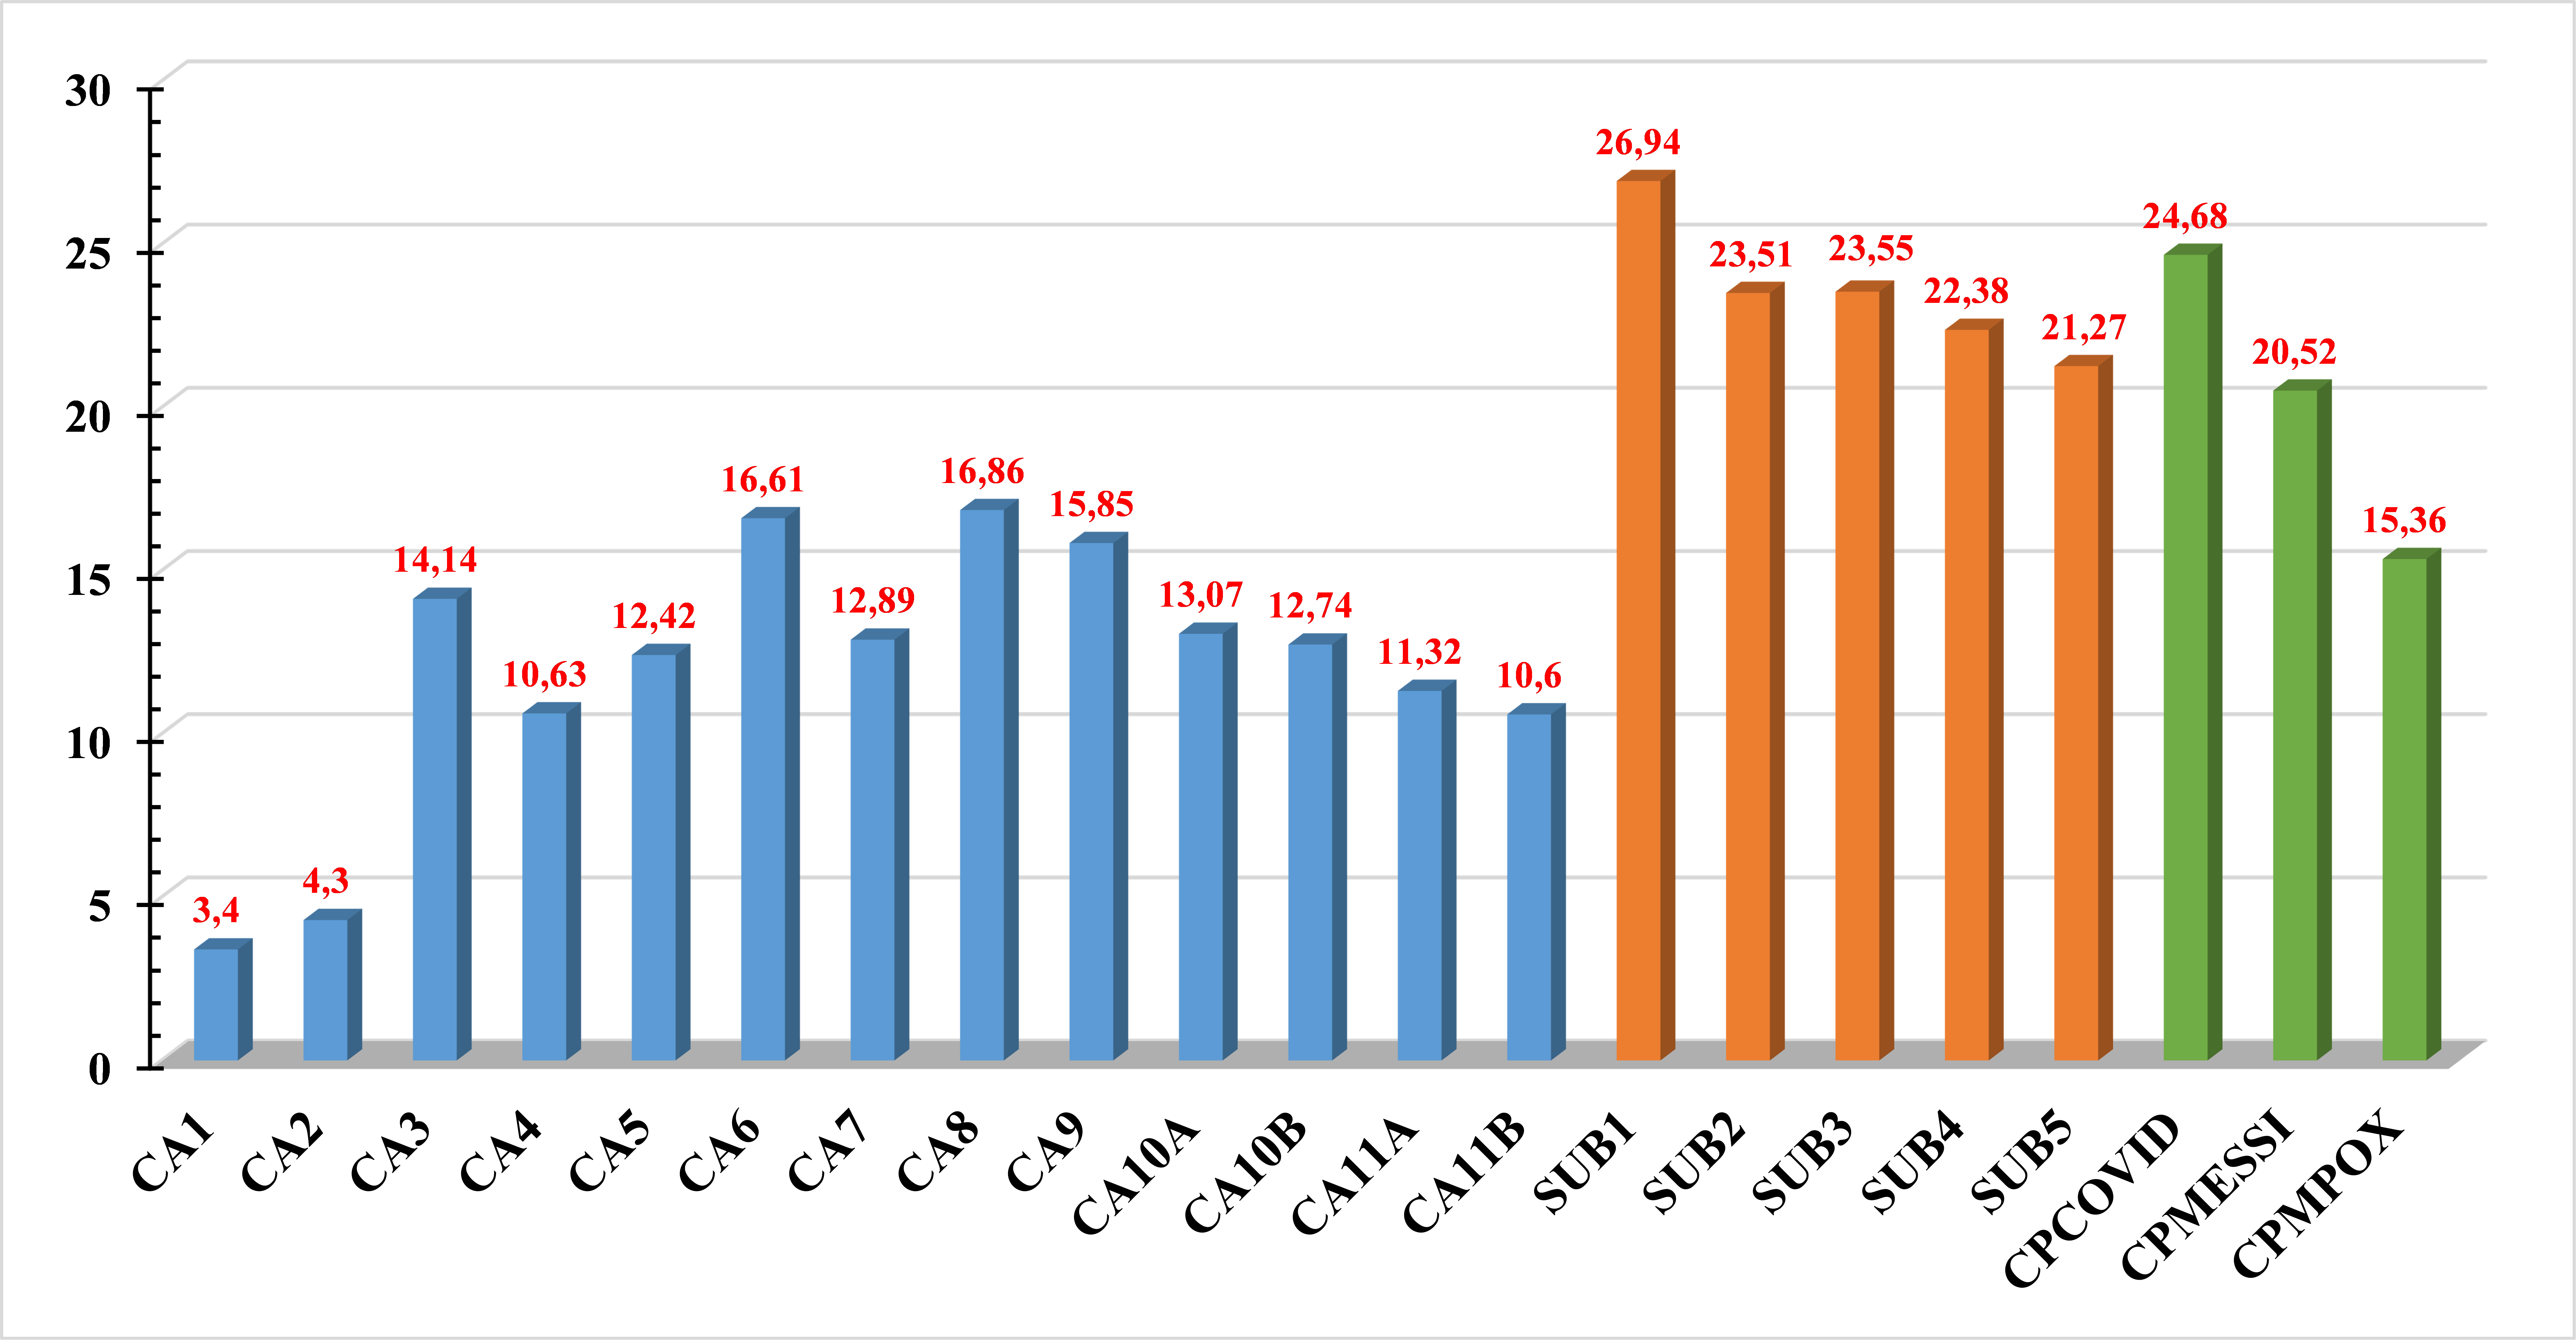
\includegraphics[width=\textwidth]{ttr.png} \caption{TTRs dos 21 (sub)corpora.} \label{fig 1}
    
\end{minipage}
    \source{Autoria própria.}
\end{figure}

É possível notar que os TTRs dos CA1 e CA2 são notadamente inferiores em comparação aos outros subcorpora do UMPLC. Por contraste, o CA3, coletado durante o segundo semestre do primeiro ano, exibe um TTR mais elevado (14,14 versus 3,4 e 4,3). Além disso, seu número de tipos de palavras é significativamente maior (1403 versus 416 e 665). Esses resultados sugerem que durante o primeiro semestre do primeiro ano, o vocabulário utilizado permanece bastante restrito, e apenas no segundo semestre os aprendizes começam a incorporar uma variedade maior de palavras em sua escrita.

Após o primeiro semestre do primeiro ano, o TTR segue um padrão oscilante: entre o momento 3 e o momento 8, o TTR flutua, atingindo o valor mais elevado no CA8. Posteriormente ao momento 8, o TTR diminui constantemente, alcançando o menor valor no CA11B. Considerando que é improvável que o conhecimento lexical dos aprendizes mude de maneira tão abrupta, argumenta-se que essa variação no TTR não reflete necessariamente o vocabulário que os estudantes dominam, mas, em vez disso, está associada aos tópicos abordados nas composições.

Em outras palavras, os tópicos podem delimitar, em maior ou menor grau, o conteúdo e, por consequência, o vocabulário nas composições, o que afeta o TTR. Se o conteúdo de um grupo de composições for altamente homogêneo, é natural que o vocabulário não apresente muita variação.

Para testar a hipótese de que a variação do TTR, conforme descrita anteriormente, está relacionada aos tópicos das composições, examinamos os tópicos das composições que compõem o CA8 e o CA11B\footnote{O tópico do CA11B utilizou dois vídeos para diferentes turmas: o vídeo\href{https://www.tdm.com.mo/pt/news-detail/590024}{"Excursões Subsidiadas"} para as turmas 1 e 2, e o vídeo \href{https://www.tdm.com.mo/pt/news-detail/590045}{"Andy Wu prevê 40 mil turistas por dia em Maio"} para as turmas 3 e 4.} (ver Tabela \ref{tab5}), ambos com números semelhantes de palavras (10821 versus 11306), mas TTRs significativamente diferentes (16,86 versus 10,6).

\begin{table}[h]
\centering
\begin{threeparttable}
\caption{Tópicos dos CA8 e CA11B}
\label{tab5}
\begin{tabular}{ll}
\toprule
O tópico das composições que compõem o CA8 & \begin{tabular}[c]{@{}l@{}}Nos últimos meses tem-se mudado muito\\ a nossa vida quotidiana devido ao surto\\ da pandemia de COVID-19. Com o fechamento \\ de escolas a nível mundial, os professores \\ e alunos tiveram de recorrer a novos \\ meios de ensino e aprendizagem, tudo à \\ distância. Como é que você vê essa mudança \\ que tem experimentado ao longo do semestre? \\ Quais são as vantagens e desvantagens? \\ Apresente a sua opinião e reflexão num texto\\ de 150-200 palavras.\end{tabular} \\
\midrule
O tópico das composições que compõem o CA11B & \begin{tabular}[c]{@{}l@{}}Após assistir ao vídeo por três vezes, \\ escreva uma notícia que resuma as suas \\ principais informações. A sua notícia \\ deve ter entre 150 e 300 palavras e \\ conter título. O subtítulo e o lead \\ são opcionais.\end{tabular}                                                                                                                                                                                                                                                \\ 
\bottomrule
\end{tabular}%
\source{Autoria própria.}
\end{threeparttable}
\end{table}

Observa-se que o tópico 8 permite uma maior flexibilidade, permitindo que os estudantes expressem suas próprias opiniões, enquanto no tópico 11B, os alunos são explicitamente instruídos a escrever um texto contendo informações específicas. Essa constatação está em conformidade com a nossa hipótese.

Para avaliar a influência do tópico no uso de vocabulário, examinamos as 10 trigramas de palavras mais frequentes (TPMFs) nos CA8 e CA11B, concentrando-nos na frequência das TPMFs e na frequência relativa de documento (FRD), ou seja, a proporção de documentos nos quais um determinado item aparece\footnote{As TPMFs e as estatísticas são extraídas utilizando o \href{https://www.sketchengine.eu/}{Sketch Engine}.} (ver Tabela \ref{tab6} e Tabela \ref{tab7}, respectivamente). 


\begin{table}[h]
\centering
\begin{threeparttable}
\caption{As 10 TPMFs no CA8}
\label{tab6}
\begin{tabular}{lll}
\toprule
Item                     & Frequência & FRD(\%)     \\ 
\midrule
ensino a distância       & 23         & 34,43        \\ 
pandemia de covid-19     & 23         & 19,67        \\ 
vantagens e desvantagens & 21         & 32,79        \\ 
surto da pandemia        & 19         & 26,23        \\ 
da pandemia de           & 17         & 24,59        \\ 
o ensino à               & 17         & 14,75        \\ 
na minha opinião         & 14         & 22,95        \\ 
ensino e aprendizagem    & 14         & 19,67        \\ 
de ensino e              & 13         & 18,03        \\ 
em casa e                & 12         & 16,39        \\ 
                         & Total: 173 & Média: 22,95 \\ 
\bottomrule
\end{tabular}
\source{Autoria própria.}
\end{threeparttable}
\end{table}

\begin{table}[h]
\centering
\begin{threeparttable}
\caption{As 10 TPMF no CA11B}
\label{tab7}
\begin{tabular}{lll}   
\toprule
Item                  & Frequência & FRD(\%)       \\ 
\midrule
serviços de turismo   & 93         & 78,57        \\ 
dos serviços de       & 79         & 71,43        \\ 
taxa média de         & 53         & 41,67        \\ 
média de ocupação     & 50         & 40,48        \\ 
helena de senna       & 49         & 48,81        \\ 
taxa de ocupação      & 45         & 36,90        \\ 
de senna fernandes    & 42         & 41,67        \\ 
de ocupação hoteleira & 41         & 34,52        \\ 
a taxa média          & 37         & 35,71        \\ 
a taxa de             & 36         & 30,95        \\ 
                      & Total: 525 & Média: 46,07 \\ 
\bottomrule
\end{tabular}
\source{Autoria própria.}
\end{threeparttable}
\end{table}



Os dados indicam que no CA11B, as 10 TPMFs são usadas proporcionalmente com maior frequência do que no CA8. Mesmo que a escala dos dois subcorpora seja semelhante, no CA11B, em média, as 10 TPMFs estão presentes em 46,07\% das composições, o que é cerca de duas vezes mais do que no CA8 (22,95\%). Além disso, a frequência total das 10 TPMFs no CA11B é consideravelmente maior (689 versus 168). Essas descobertas corroboram a hipótese de que um tópico com mais restrições pode resultar em um uso lexical mais limitado e repetitivo.

Uma análise mais detalhada das TPMFs revela que, essencialmente, elas ecoam os tópicos abordados, visto que quase todas essas trigramas podem ser encontradas nos tópicos ou materiais relacionados. Isso sugere que as composições dos estudantes, além de expressar suas próprias ideias, incorporam, em diferentes graus, a linguagem daqueles que elaboram os materiais \cite{kreyer2017multilinguality}. Esse fenômeno, mais uma vez, ilustra a influência dos tópicos nas composições dos alunos.

A partir dessas constatações, pode-se argumentar que a variação do TTR está intrinsecamente associada aos tópicos abordados nas composições. Ao avaliar as composições dos aprendizes, é importante interpretar o TTR com cautela, uma vez que um TTR mais baixo não necessariamente indica um domínio lexical inferior. No entanto, o TTR ainda fornece um ponto de referência para avaliar o conhecimento lexical dos aprendizes, permitindo uma visão geral da evolução diacrônica da variação lexical, especialmente quando o progresso é evidente, como demonstrado na comparação entre o CA1, o CA2 e o CA3.

A seguir, conduzimos análises quantitativas com o objetivo de investigar possíveis diferenças na variação lexical entre os subcorpora do UMPLC e os (sub)corpora de referência (ptTenTen20, CPCOVID, CPMESSI e CPMPOX). Em comparação com os subcorpora do UMPLC, os do ptTenTen20 exibem TTRs significativamente mais elevados: no primeiro grupo, a média do TTR é de 11,91\%, enquanto no último, a média é de 23,02\%. Em relação ao número de tipos de palavras, o menor subcorpus do ptTenTen20 (SUB1) contém mais tipos do que a maioria dos subcorpora do UMPLC.

Esses dados indicam que as composições apresentam um nível de variação lexical mais baixo do que os textos produzidos por falantes nativos. No entanto, como já mencionado, o TTR representa a diversidade de vocabulário em uso, o qual, por sua vez, pode ser influenciado pelos temas abordados. Portanto, a discrepância do TTR entre esses dois tipos de subcorpora, em vez de refletir uma diferença genuína no conhecimento lexical entre falantes nativos e não nativos, pode ser atribuída ao fato de que, ao contrário das composições que se concentram em um tópico específico, os textos do ptTenTen20 abrangem uma ampla variedade de tópicos.

Para uma análise mais aprofundada das razões subjacentes à diferença na variação lexical mencionada anteriormente, contrastamos os subcorpora do UMPLC com o CPCOVID, o CPMESSI e o CPMPOX. Esses três \textit{corpora} foram construídos em torno de palavras-chave específicas, resultando em conteúdo mais homogêneo em comparação com os subcorpora do ptTenTen20, que consistem em textos aleatórios. Entre os três corpora, o conteúdo do CPCOVID provavelmente é o menos homogêneo, uma vez que as notícias frequentemente abordam tópicos variados, como a reintrodução de máscaras, novas variantes e o cancelamento de políticas relacionadas à pandemia. Em contrapartida, o CPMESSI e o CPMPOX devem possuir um conteúdo mais concentrado, já que o primeiro se concentra principalmente na vitória de Leo Messi na Copa das Ligas, e o segundo aborda os surtos recentes de Mpox em Portugal. Para quantificar o grau de homogeneidade, calculamos a média da Frequência Relativa de Documento (FRD) das 10 TPMFs (ver Tabela \ref{tab8}). Os resultados indicam que essa métrica corresponde bem às avaliações subjetivas mencionadas neste parágrafo.


\begin{table}[h]
\centering
\begin{threeparttable}
\caption{Média da FRD das 10 TPMFs dos CPCOVID, CPMESSI e CPMPOX}
\label{tab8}
\begin{tabular}{ll}
\toprule
Corpus  & \begin{tabular}[c]{@{}l@{}}Média da FRD \\ das 10 TPMFs\end{tabular} \\
\midrule
CPCOVID & 29,23                                                                \\
CPMESSI & 49,09                                                                \\
CPMPOX  & 55,83                                                                \\
\bottomrule
\end{tabular}
\source{Autoria própria.}
\end{threeparttable}
\end{table}

A partir da média da FRD das 10 TPMFs, nota-se que o nível de homogeneidade nos CA11B, CPMESSI e CPMPOX é essencialmente equivalente, com o CA11B apresentando uma média da FRD ligeiramente inferior em comparação com os outros dois \textit{corpora} (46,07\% versus 49,09\% e 55,83\%). Da mesma forma, o CA8 e o CPCOVID exibem um nível de homogeneidade semelhante, uma vez que as médias da FRD das 10 TPMFs não diferem significativamente (22,95\% \textit{versus} 29,23\%).

Com base nesses dados, podemos concluir que o vocabulário dos CPMESSI e CPMPOX é mais diversificado em comparação com o do CA11B, e o vocabulário do CPCOVID é mais variado do que o do CA8. Isso fica claramente evidente quando se analisa o TTR: o TTR nos CPMESSI e CPMPOX é aproximadamente duas e uma vez e meia maior do que o do CA11B, respectivamente (20,52\% e 15,36\% versus 10,6\%), enquanto o TTR do CPCOVID é cerca de uma vez e meia maior do que o do CA8 (24,68\% versus 16,86\%). Além disso, o número de tipos de palavras nos CPMESSI, CPMPOX e CPCOVID também é maior, apesar de o CA11B e o CA8 conterem mais palavras no total. Isso sugere que, em condições semelhantes, os aprendizes utilizam um vocabulário menos variado em comparação com os falantes nativos.

Em resumo, a partir das análises apresentadas, podemos chegar a três conclusões. Primeiro, para os estudantes em questão, o primeiro semestre do 1º ano é o período em que o uso de vocabulário permanece mais limitado; somente após esse período eles começam a ser capazes de utilizar palavras mais diversificadas em sua escrita. Segundo, a variação no TTR observada nos subcorpora CA3 a CA11B parece estar relacionada à influência dos tópicos abordados, e não reflete uma mudança real no conhecimento lexical dos estudantes. Terceiro, os dados da comparação entre os subcorpora do UMPLC e os subcorpora de referência revelam que os aprendizes chineses de português L2 não escrevem com o mesmo nível de variação lexical que os falantes nativos.

\section{Estudo II: advérbios “especialmente” e “nomeadamente”}

Nesta seção, nossa intenção é investigar, tanto quantitativamente quanto qualitativamente, o uso de advérbios que apresentam o sufixo "mente". É importante destacar que a categoria gramatical dos advérbios não costuma ser facilmente confundida com outras categorias nos sistemas de anotação.

Inicialmente, procedemos à análise dos advérbios terminados em "mente" nos subcorpora \textit{Portuguese TLD} (PT) e \textit{Brazilian TLD} (BT) - dois subconjuntos presentes no ptTenTen20 que representam o português europeu e o brasileiro, respectivamente. Essa investigação teve como objetivo identificar padrões e fenômenos intrigantes que merecessem uma investigação mais aprofundada. Verificamos que o advérbio "especialmente" é um dos mais frequentemente empregados entre os advérbios com essa terminação em ambos os subcorpora.

Além disso, notamos que o advérbio "nomeadamente" é o mais comum entre os advérbios terminados em "mente" no PT, mas sua ocorrência é consideravelmente menor no BT. Realizamos um teste qui-quadrado, constatando que "nomeadamente" é significativamente mais frequente no PT em comparação ao BT (\(\chi\)\(^2\) = 1501677, df = 1, p < 0,001). Os dados relevantes estão apresentados na Tabela \ref{tab9}.


\begin{table}[h]
\centering
\begin{threeparttable}
\caption{"Especialmente" e "Nomeadamente" nos PT e BT}
\label{tab9}
\begin{tabular}{lcccc}
\hline
\multirow{2}{*}{} & \multicolumn{2}{c}{Especialmente}                                                     & \multicolumn{2}{c}{Nomeadamente} \\ %\cline{2-5} 
                  & Frequência & Frequência Relativa$^\dagger$ & Frequência & Frequência Relativa \\ 
		  \midrule
PT                & 77113      & 102,32                                                                   & 181802     & 241,24              \\ 
BT                & 809578     & 120,36                                                                   & 11809      & 1,76                \\ 
\bottomrule
\end{tabular}
\source{Autoria própria.}
\notes{$\dagger$ Frequência por um milhão de palavras.}
\end{threeparttable}
\end{table}

A seguir, examinamos os advérbios terminados em “mente” no UMPLC. Neste corpus de aprendizes, o advérbio "especialmente" é muito mais frequente do que "nomeadamente" - o primeiro aparece 62 vezes, enquanto o último ocorre apenas 4 vezes. O português europeu é a variante usada em Macau. Levando isso em consideração, nesta seção, o UMPLC será comparado com o PT, em vez do BT.

Para determinar se há uma diferença quantitativa estatisticamente significativa entre os dois advérbios no UMPLC e no PT, conduzimos dois testes estatísticos: um teste qui-quadrado e um teste g. O teste qui-quadrado indica que, em relação ao PT, o "especialmente" é utilizado de forma significativamente mais frequente no UMPLC (\(\chi\)\(^2\)=109,52, df=1, p<0,001). Já o teste g revela que, comparado ao PT, o "nomeadamente" é empregado de maneira significativamente menos frequente no UMPLC (G=56,236, df=1, p<0,001).

Com o objetivo de realizar uma análise detalhada dos dois advérbios, examinamos seus usos e classificamos esses advérbios com base no sentido que eles assumem no contexto. Primeiramente, apresentamos a análise referente ao advérbio "especialmente".

De acordo com dois dicionários online\footnote{\href{https://www.aulete.com.br}{Aulete} e \href{https://www.infopedia.pt/dicionarios/lingua-portuguesa}{Infopédia}.}, o advérbio “especialmente” tem cinco significados: A. muito, bastante, B. somente para um certo fim, objetivo ou propósito, C. apenas para uma certa pessoa ou para um certo grupo de pessoas, D. em consideração ou na intenção de, E. de um modo mais especial, acima de tudo, sobretudo, principalmente. Os resultados da análise indicam que no UMPLC, o uso deste advérbio é bastante restrito, sendo utilizado principalmente com dois significados: o significado E é predominante, representando 96,77\% dos casos, enquanto o significado A aparece apenas duas vezes. Essas informações são apresentadas na Tabela \ref{tab10}.

\begin{table}[h]
\centering
\begin{threeparttable}
\caption{Distribuição do "Especialmente" no UMPLC}
\label{tab10}
\begin{tabular}{lll}
\toprule
Significado & Frequência & Percentagem \\ 
\midrule
A           & 2          & 3,32        \\ 
B           & 0          & 0           \\ 
C           & 0          & 0           \\ 
D           & 0          & 0           \\ 
E           & 60         & 96,77       \\ 
\bottomrule
\end{tabular}
\source{Autoria própria.}
\end{threeparttable}
\end{table}

Para avaliar se essa concentração também é observada na escrita dos falantes nativos, foram aleatoriamente selecionadas 50 frases contendo o advérbio "especialmente" do PT. Essas frases foram classificadas utilizando o mesmo método, e os resultados são apresentados na Tabela \ref{tab11}. Pode-se notar que, nessa amostra, o advérbio também é predominantemente utilizado com o significado E. No entanto, o uso é relativamente mais diversificado em comparação com o UMPLC, abrangendo quatro significados distintos.

\begin{table}[h]
\centering
\begin{threeparttable}
\caption{Distribuição do "Especialmente" na Amosta do PT}
\label{tab11}
\begin{tabular}{lll}
\toprule
Significado & Frequência & Percentagem \\ 
\midrule
A           & 6          & 12          \\ 
B           & 1          & 2           \\ 
C           & 0          & 0           \\ 
D           & 5          & 10          \\ 
E           & 38         & 76          \\ 
\bottomrule
\end{tabular}
\source{Autoria própria.}
\end{threeparttable}
\end{table}

Além dessa diferença, observou-se que no UMPLC, o uso do advérbio "especialmente" apresenta uma característica notável: o advérbio frequentemente é colocado no início das frases (9 vezes), enquanto na amostra do PT, ele aparece quase sempre no meio das frases (49 vezes). Para uma melhor compreensão desse fenômeno, investigamos o uso de "especialmente" no PT e descobrimos que, das 77113 ocorrências, o advérbio aparece apenas 3331 vezes no início das frases (4,32\%).

Com base nesses dados, realizamos um teste g, cujo resultado (G = 9,8604, df = 1, p < 0,01) indica que o "especialmente" é colocado significativamente com mais frequência no início das frases no UMPLC em comparação com o PT.

Suscita-se a hipótese de que a tendência dos aprendizes chineses de colocarem o advérbio "especialmente" mais frequentemente no início das frases decorre da interferência negativa da língua chinesa, já que "yóu qí shì" e "tè bié shì" (duas possíveis traduções para "especialmente") aparentam ocorrer com frequência na posição inicial das sentenças em chinês. Para testar essa hipótese, realizamos uma pesquisa nas duas expressões chinesas no \textit{corpus} zhTenTen17 e constatamos que "yóu qí shì" ocorre 1653524 vezes, sendo que 16,93\% delas (279915) estão no início das sentenças, enquanto "tè bié shì" ocorre 1293428 vezes, com 25,36\% delas (328032) no início das sentenças.

Para avaliar se existe uma diferença quantitativa estatisticamente significativa na ocorrência de "especialmente", "yóu qí shì" e "tè bié shì" no início das frases, conduzimos quatro testes de qui-quadrado. As comparações entre o PT e o corpus zhTenTen17 indicam que tanto "yóu qí shì" (\(\chi\)\(^2\)=8556,4, df=1, p<0,001) quanto "tè bié shì" (\(\chi\)\(^2\)=17575, df=1, p<0,001) ocorrem significativamente mais frequentemente no início das sentenças em comparação com "especialmente" no PT.

Por outro lado, as comparações entre o UMPLC e o \textit{corpus} zhTenTen17 demonstram que "yóu qí shì" (\(\chi\)\(^2\)=0,11368, df=1, p=0,736 > 0,05) e "tè bié shì" (\(\chi\)\(^2\)=3,3007, df=1, p=0,06925 > 0,05) no zhTenTen17 não ocorrem com maior frequência no início das sentenças em comparação com "especialmente" no UMPLC. Em resumo, no zhTenTen17, "yóu qí shì" e "tè bié shì" são mais frequentemente usados no início das sentenças do que "especialmente" no PT, e essas mesmas expressões chinesas apresentam uma taxa similar de ocorrência no início das sentenças em comparação com "especialmente" no UMPLC.


Com base nesses resultados, é possível afirmar que a tendência dos aprendizes de colocar "especialmente" no início das sentenças é resultado da interferência da língua chinesa.

O advérbio "nomeadamente" foi analisado de maneira semelhante. Identificamos sentenças contendo esse advérbio no UMPLC e, em seguida, categorizamos seu uso de acordo com os significados listados nos dicionários mencionados anteriormente: A. dando nome a, indicando o nome de, com ou segundo declinação dos nomes, B. mais exatamente, mais especificamente C. principalmente, mormente. No UMPLC, encontramos apenas quatro ocorrências de "nomeadamente", das quais três apresentam o significado C. e uma inclui um erro inexplicável. Isso sugere que os aprendizes não estão familiarizados com o uso desse advérbio. Com base nos três casos em que o advérbio é corretamente empregado, é possível deduzir que os estudantes simplesmente o consideram um sinônimo de "especialmente", utilizando-o apenas para destacar informações específicas.   

Foram aleatoriamente selecionadas 50 sentenças contendo a palavra "nomeadamente" do PT e analisadas (ver Tabela \ref{tab12}). Os resultados evidenciam que, para os falantes nativos, "nomeadamente" é principalmente utilizado para detalhar informações (significado B). Em outras palavras, o uso desse advérbio é diferente no PT em comparação com o UMPLC.

\begin{table}[h]
\centering
\begin{threeparttable}
\caption{Distribuição do "Nomeadamente" na Amosta do PT}
\label{tab12}
\begin{tabular}{lll}
\toprule
Significado & Frequência & Percentagem \\ 
\midrule
A           & 1          & 2           \\ 
B           & 46         & 92          \\ 
C           & 3          & 6           \\ 
\bottomrule
\end{tabular}
\source{Autoria própria.}
\end{threeparttable}
\end{table}

Nesta seção, investigamos de forma contrastiva dois advérbios terminados em "mente" - "especialmente" e "nomeadamente". As análises quantitativas revelaram que, em comparação com os textos produzidos por falantes nativos de português, no UMPLC, o advérbio "especialmente" apresenta uma frequência significativamente mais alta. Por outro lado, o "nomeadamente" é extremamente subutilizado.

Além das análises quantitativas, também realizamos análises qualitativas. Ao examinarmos o contexto de uso desses advérbios, constatamos que os aprendizes os utilizam de maneira diferente em comparação com os falantes nativos de português europeu. No UMPLC, o uso de "especialmente" é mais uniforme e, frequentemente, é colocado no início das frases, o que resulta da influência negativa do chinês, língua materna dos aprendizes.

A comparação entre o UMPLC e o PT sugere que os aprendizes provavelmente não estão familiarizados com o uso de "nomeadamente". No UMPLC, esse advérbio não apenas é pouco utilizado, mas também é empregado de maneira diferente em relação ao seu uso pelos falantes nativos de português europeu.

\section{Discussões finais}\label{sec-conclusao}

O UMPLC é o primeiro \textit{corpus} exclusivamente focado em falantes chineses de português L2, composto por dados longitudinais gerados em um contexto formal de ensino superior. Todos os dados são anotados com informações linguísticas, divididas em duas estruturas: \textit{PoS} e lema. Atualmente, a pesquisa está na fase final de construção da plataforma na qual o corpus e ferramentas de pesquisa \textit{online} serão disponibilizados.

Neste texto, foram apresentados os resultados de dois estudos preliminares relacionados ao uso lexical de aprendizes chineses de português L2, com base no UMPLC.  

O primeiro estudo abordou a variação lexical, que se refere à diversidade de palavras e expressões utilizadas pelos aprendizes. Essa variação reflete não apenas o nível de proficiência, mas também as influências culturais e linguísticas enfrentadas pelos estudantes ao aprender uma língua estrangeira. Os resultados revelam que os aprendizes chineses começaram a apresentar um aumento notável na variação lexical durante o segundo semestre do primeiro ano. Essa descoberta auxiliará os professores na compreensão do desenvolvimento da proficiência linguística dos aprendizes e na expansão de seu vocabulário, levando em consideração essa característica.

Isso ressalta a importância, a partir desta fase de ensino-aprendizagem, de os professores incentivarem ainda mais a leitura e a escrita entre os aprendizes chineses, expondo-os a uma ampla gama de palavras e expressões em português. Além disso, podem motivá-los a escrever mais, praticando o uso correto do vocabulário.

Além disso, observou-se que os tópicos de composição estão intimamente ligados à variação lexical dos aprendizes. Portanto, ao avaliar a competência na produção escrita dos estudantes por meio de suas composições, é essencial definir os tópicos de maneira ampla e genérica para melhor compreender seu domínio vocabular.

A pesquisa revela também que os aprendizes chineses de português L2 não atingem o mesmo nível de variação lexical observado em falantes nativos. Conscientes dessa diferença, os professores podem adaptar seus materiais didáticos, direcionando-se para as áreas onde os estudantes apresentam lacunas no vocabulário. Além disso, podem desenvolver atividades e tarefas específicas para aprimorar a proficiência vocabular dos aprendizes, ao mesmo tempo em que sensibilizam os alunos para as nuances linguísticas presentes em contextos sociais e culturais.

Assim, os resultados da pesquisa sobre a variação lexical no contexto do UMPLC fornecem \textit{insights} valiosos para a avaliação e aprimoramento do ensino de português L2. Os professores podem empregar essas descobertas para adaptar seu ensino de forma personalizada e auxiliar os estudantes a alcançarem um patamar superior de proficiência linguística e competência comunicativa.

Além disso, os resultados do segundo estudo demonstram a transferência negativa da língua materna e o fenômeno de sobreutilização e subutilização no uso de advérbios em português por parte dos aprendizes chineses. Essa análise é valiosa porque identifica padrões de uso inadequado em comparação com os falantes nativos, o que pode oferecer \textit{insights} importantes para o ensino e aprendizagem eficazes. A compreensão de como os aprendizes utilizam advérbios, suas tendências de sobreutilização e subutilização, bem como a comparação com o uso nativo da língua, capacita os professores a desenvolverem estratégias pedagógicas mais direcionadas e a adaptar os materiais didáticos de maneira a atender às necessidades específicas dos aprendizes. 

Os exemplos das aplicações pedagógicas demonstram que o UMPLC é de extrema relevância, pois constitui um recurso essencial para uma compreensão mais aprofundada da interlíngua dos aprendizes chineses, servindo como uma base empírica sólida para o desenvolvimento do ensino de português L2.

Por meio desta pesquisa, adquirimos uma compreensão mais sólida da importância da tecnologia, mais especificamente, da tecnologia relacionada a \textit{corpora}, no contexto do ensino de L2. O UMPLC, cuja construção está em fase final, em breve estará disponível para pessoas registradas interessadas em utilizá-lo para fins de pesquisa. Estamos confiantes de que o UMPLC se tornará uma ferramenta amplamente utilizada no campo do ensino e da pesquisa em português L2.

\section{Financiamento}
O presente estudo foi desenvolvido no âmbito de MYRG2020-00139-FAH e de SRG2020-00021-FAH, projetos financiados pela Universidade de Macau.

\printbibliography\label{sec-bib}

\begin{contributors}[sec-contributors] \authorcontribution{Jing Zhang}[conceptualization, projadm, investigation, methodology, writing, review]


\authorcontribution{Mu You}[datacuration, formalanalysis, methodology, writing, review]
\end{contributors}


\end{document}

